\documentclass[11pt]{article}

\usepackage{graphicx}
\usepackage{amsmath}
\usepackage{amssymb}
\usepackage{color}
\usepackage{listings}
\usepackage{xcolor}

\definecolor{codegreen}{rgb}{0,0.6,0}
\definecolor{codegray}{rgb}{0.5,0.5,0.5}
\definecolor{codepurple}{rgb}{0.58,0,0.82}
\definecolor{backcolour}{rgb}{0.95,0.95,0.92}

\lstdefinestyle{mystyle}{
    backgroundcolor=\color{backcolour},   
    commentstyle=\color{codegreen},
    keywordstyle=\color{magenta},
    numberstyle=\tiny\color{codegray},
    stringstyle=\color{codepurple},
    basicstyle=\ttfamily\footnotesize,
    breakatwhitespace=false,         
    breaklines=true,                 
    captionpos=b,                    
    keepspaces=true,                 
    numbers=left,                    
    numbersep=5pt,                  
    showspaces=false,                
    showstringspaces=false,
    showtabs=false,                  
    tabsize=2
}

\lstset{style=mystyle}

\textwidth=6.5in
\textheight=9in
\topmargin=-0.8in
\headheight=15.75pt
\headsep=.35in
\oddsidemargin=0.0in
\evensidemargin=0.0in

\newcommand{\Complex}{\mathbb{C}}
\newcommand{\Real}{\mathbb{R}}
\newcommand{\Dpt}{D_{+t}}
\newcommand{\Dmt}{D_{-t}}
\newcommand{\Dzt}{D_{0t}}
\newcommand{\Dpx}{D_{+x}}
\newcommand{\Dmx}{D_{-x}}
\newcommand{\Dzx}{D_{0x}}
\newcommand{\Oc}{\mathcal{O}}
\newcommand{\dx}{\Delta x}
\newcommand{\dy}{\Delta y}
\newcommand{\dt}{\Delta t}
\newcommand{\ut}{u_t}
\newcommand{\uxx}{u_{xx}}
\newcommand{\uyy}{u_{yy}}
\newcommand{\vnpjm}{v^{n+1}_{j-1}}
\newcommand{\vnpjp}{v^{n+1}_{j+1}}
\newcommand{\vnpj}{v^{n+1}_{j}}
\newcommand{\vnjm}{v^{n}_{j-1}}
\newcommand{\vnjp}{v^{n}_{j+1}}
\newcommand{\vnj}{v^{n}_{j}}
\newcommand{\vhnp}{\hat{V}^{n+1}}
\newcommand{\vhn}{\hat{V}^n}
\newcommand{\bra}[1]{\left(#1\right)}

\begin{document}
\begin{flushright}
\small{MATH-6840\\
Vignesh Ramakrishnan\\
RIN: 662028006 \\
{\bf Due: Monday March 21, 2022}}
\end{flushright}

\begin{center}
\large{Problem Set 6}\\
\end{center}

\begin{enumerate}
  %%%%%
  %%%%%
  %%%%%
  \item (25 pts.) Consider the advection-diffusion equation
    \begin{align*}
      u_t+au_x- \nu u_{xx} & =f(x,t), \qquad x\in(0,1), \qquad 0 < t \le T_f\\
      u(x,0) & = u_0(x), \qquad x\in(0,1)\\
      u(0,t) & = \alpha(t), \qquad \\
      u_x(1,t) & = \beta(t), \qquad t\ge 0 \qquad t\ge 0.
    \end{align*}
    %
    \begin{enumerate}
      \item {\color{red}Determine $f(x,t)$, $u_0(x)$, $\alpha(t)$, and $\beta(t)$ so that the exact solution to the problem is $u(x,t)=2\cos(3x)\cos(t)$.}
      \begin{align*}
      u_{ex}(x,t) =& \ 2\cos(3x)\cos(t) \\
      \ut(x,t) =& \ -2\cos(3x)\sin(t) \\
      u_x(x,t) =& \ -6\sin(3x)\cos(t) \\
      \uxx(x,t) =& \ -18\cos(3x)\cos(t) \\
      \ut + a u_x -\nu \uxx =& \ \cos(3x)\left[18\nu\cos(t) -2\sin(t)\right] -6a\sin(3x)\cos(t) = f(x,t) \\
      u(x,t=0) =& \ 2\cos(3x) = u_0(x,t=0) \\
      u(x=0,t) =& \ 2\cos(t) = \alpha(t) \\
      u_x(x=1,t) =& \ -6\sin(3)\cos(t) = \beta(t)
      \end{align*}
      %
      \item {\color{red}Now using the computational grid defined by $x_j=j\Delta x$, $-1,0,\ldots,N+1$, with $\Delta x=1/N$ (note there is a ghost cell at left and right), define a discrete treatment of the boundary conditions that is at least second-order accurate.} 
      \begin{align*}
      x_j =& \ j\Delta x, \; j = -1,0,1,2,\ldots \ldots, N_x, N_x +1 \\
      v^{n+1}_0 =&\ \frac{v^{n+1}_{-1} + v^{n+1}_1}{2} = 2\cos(t^{n+1})\\
      -6\sin(3)\cos(t^{n+1}) =& \ \Dzx v^{n+1}_{N_x} = \frac{v^{n+1}_{N_x + 1}-v^{n+1}_{N_x - 1}}{2\dx}
      \end{align*}
      %
      \item {\color{red}Write a code to solve this problem using the Crank-Nicolson scheme}
        \[
          \Dpt v_j^n = \left(-a\Dzx+\nu \Dpx\Dmx\right)\frac{v_j^{n+1}+v_j^n}{2}+\frac{f_j^{n+1}+f_j^n}{2}.
        \]
        {\color{red}for all interior $j$ (exact values may depend on your discrete BCs), along with the BCs you defined in part (b) above.}\\
        When the scheme is worked out, the final discretization has the form:
        \begin{align*}
        -\bra{\frac{r}{2} + \frac{\sigma}{4}}\vnpjm + &\bra{1+r}\vnpj -\bra{\frac{r}{2} - \frac{\sigma}{4}}\vnpjp = \\
        & \ \bra{\frac{r}{2} + \frac{\sigma}{4}}\vnjp + \bra{1-r}\vnj + \bra{\frac{r}{2} - \frac{\sigma}{4}}\vnjp +\frac{f^{n+1}_j + f^n_j}{2} \\
        & , \; j=0,1,2,3,\ldots \ldots N_x 
        \end{align*}
        where, $r=\frac{\nu\dt}{\dx^2}$ and $\sigma = \frac{a\dt}{\dx}$. The code is attached below in Listing~\ref{lst:CN_AD}.
        \lstinputlisting[caption={Crank-Nicholson scheme - AD Equation},label={lst:CN_AD},language=Octave]{ADCrankNicholson.m}
      %
      \item {\color{red}Perform a grid refinement study with $a=1$, $\nu=1$, and $\Delta t = \Delta x$. Present results for the maximum error in the approximation at $t=1$. Discuss the observed order-of-accuracy.} \\
      The scheme developed initially converges at an order $\approx \mathcal{O}(\dx^2)$.
      \begin{figure}[htp]
      \centering
      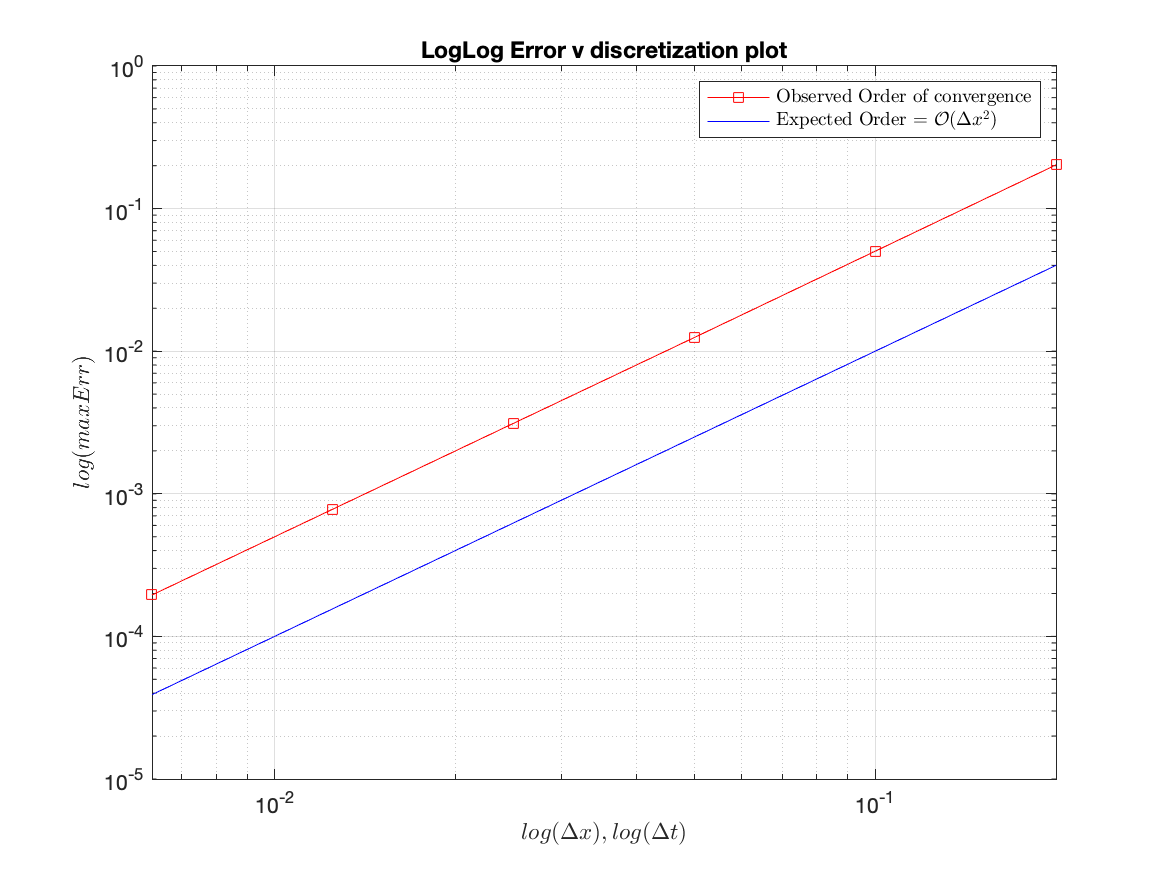
\includegraphics[width=5in]{ErrPlotQ1.png}
      \caption{Grid Refinement - LogLog plot}
      \label{fig:q1_1}
      \end{figure}
      
      \begin{figure}[htp]
      \centering
      \begin{tabular}{cc}
      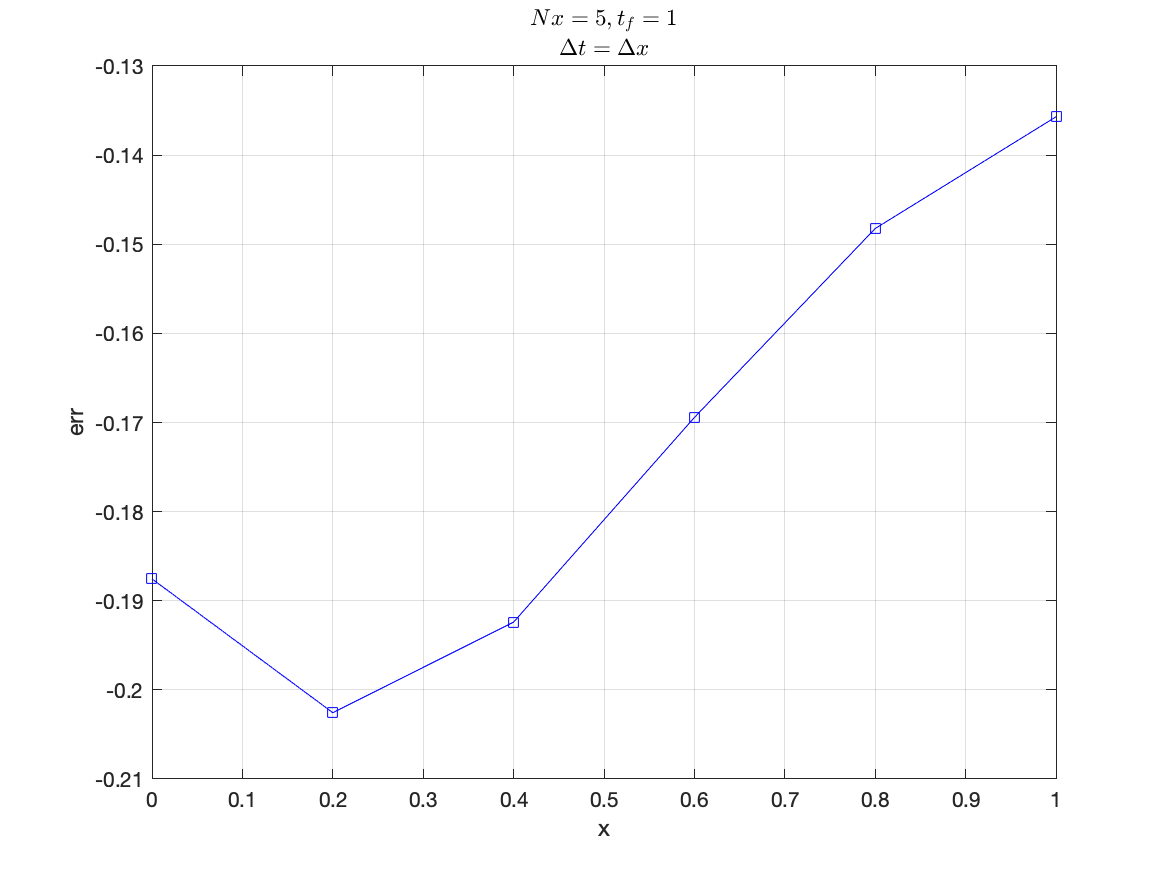
\includegraphics[width=3.3in]{ErrVx_1.png} & 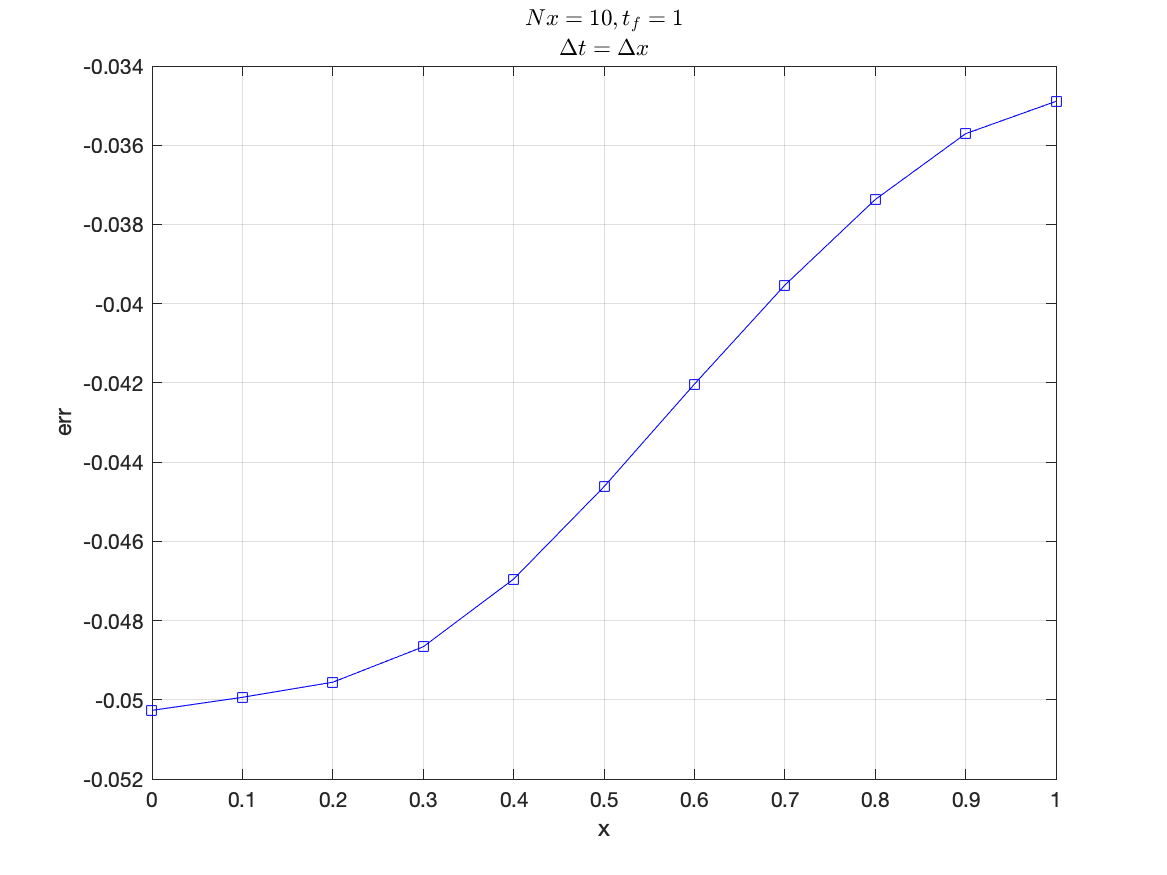
\includegraphics[width=3.3in]{ErrVx_2.png} \\
      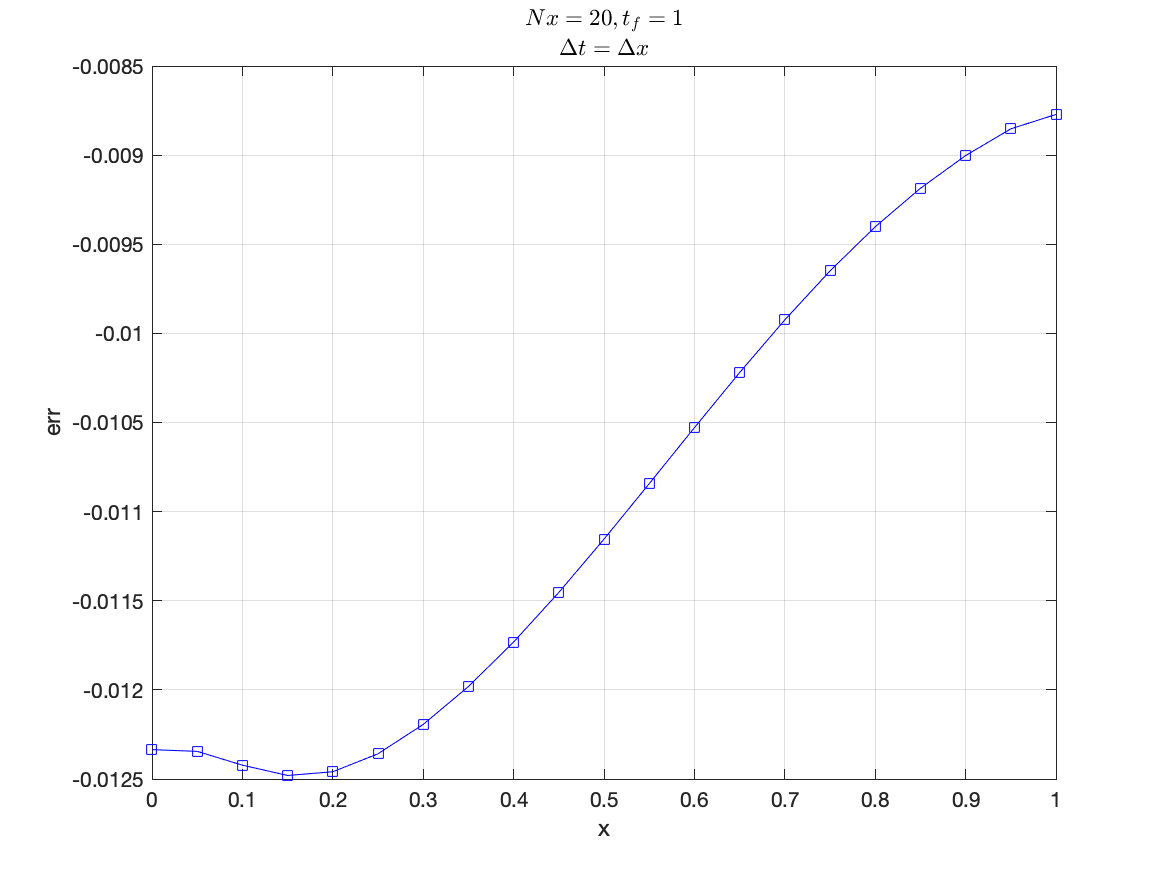
\includegraphics[width=3.3in]{ErrVx_3.png} & 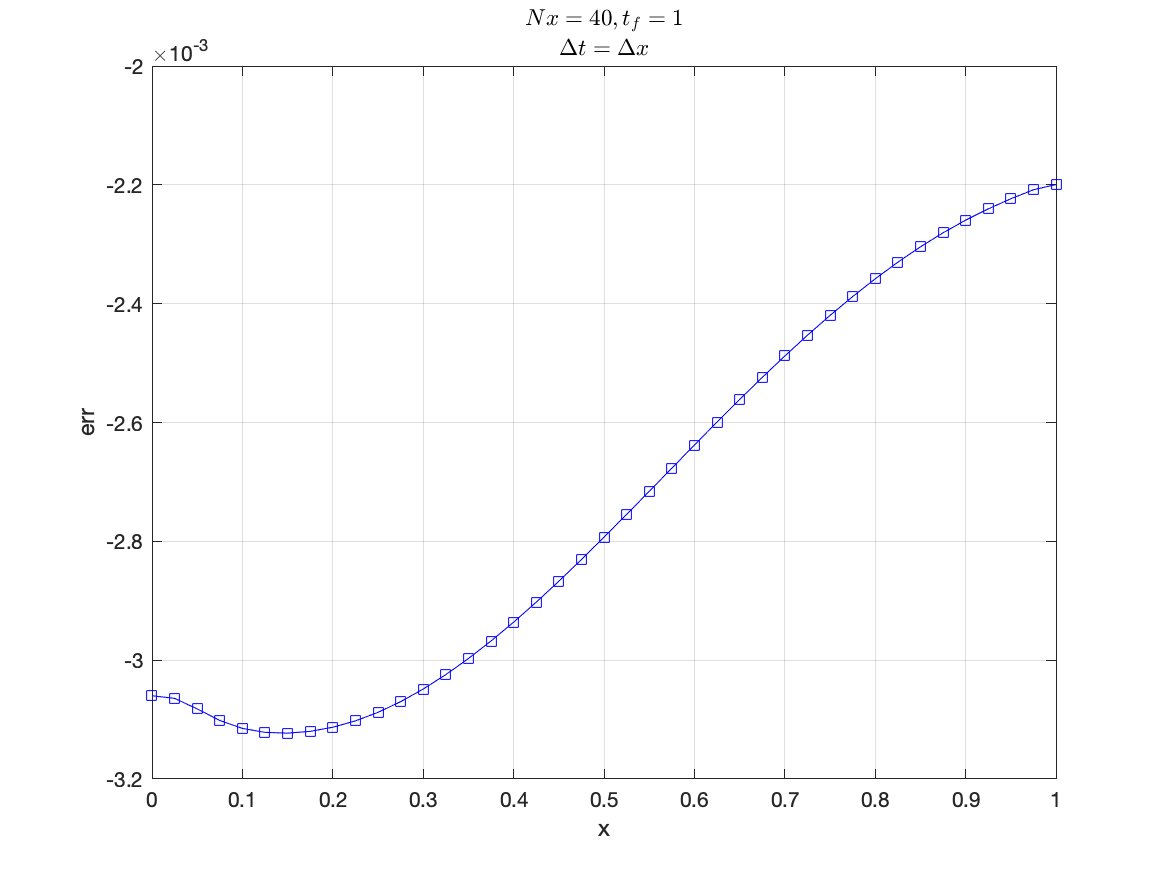
\includegraphics[width=3.3in]{ErrVx_4.png}\\
      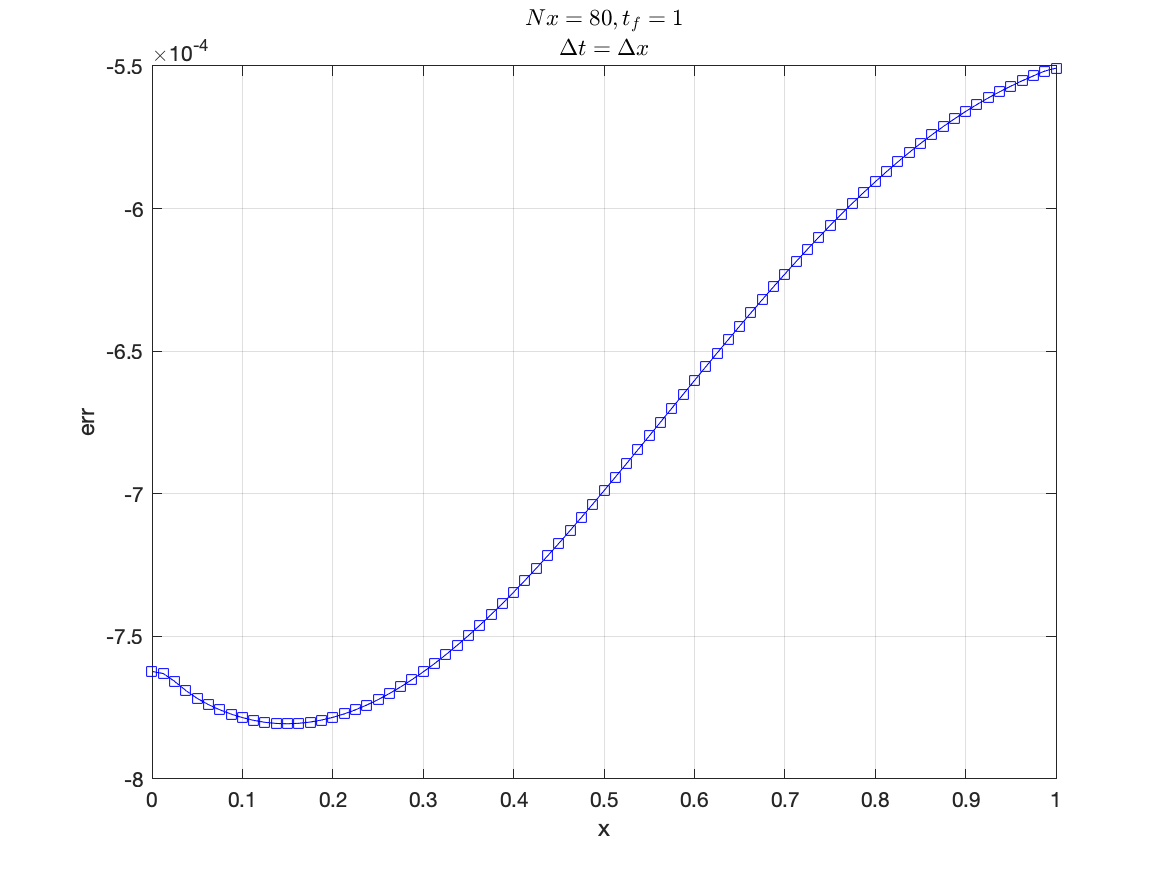
\includegraphics[width=3.3in]{ErrVx_5.png} & 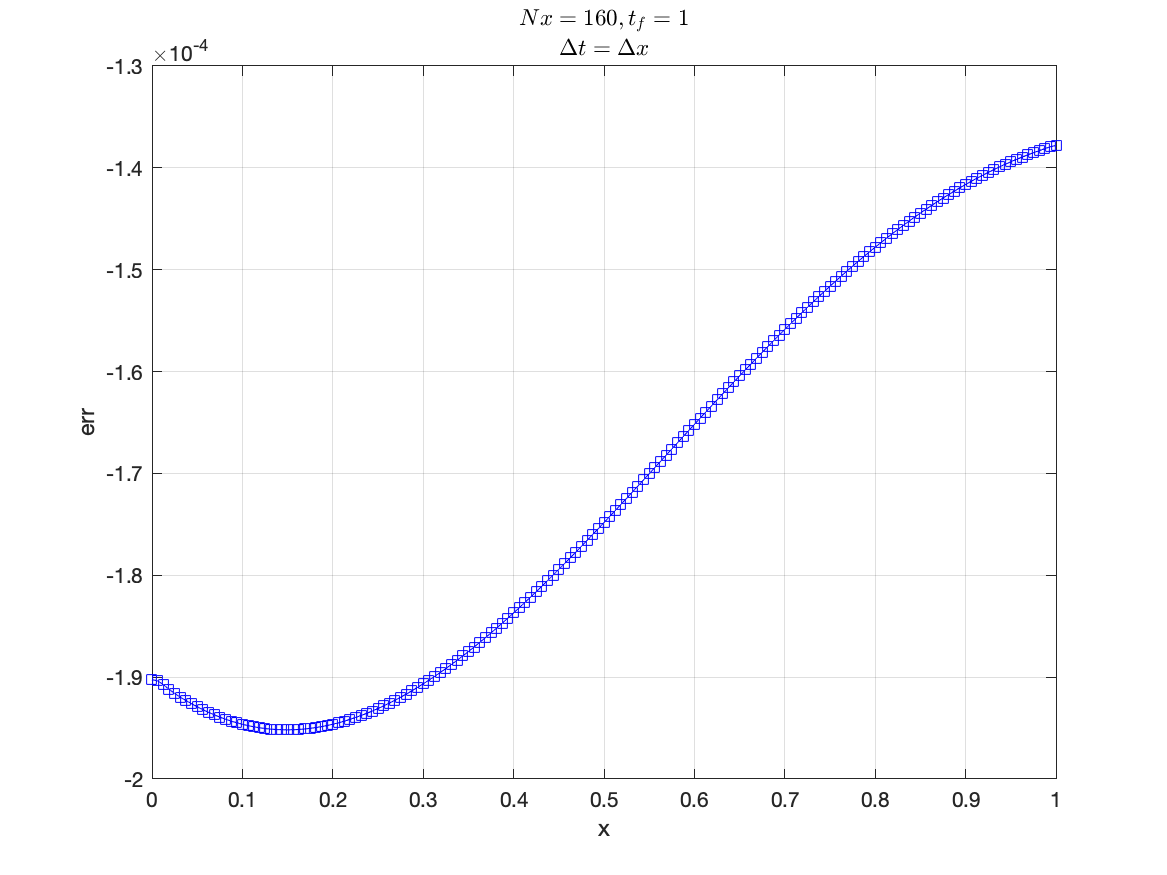
\includegraphics[width=3.3in]{ErrVx_6.png}
      \end{tabular}
      \caption{Error Plot v x}
      \label{fig:q1_2}
      \end{figure}
      
      \item {\color{red}In your computations, you should have observed stability for $\Delta t = \Delta x$. Perform a stability analysis for the Cauchy problem (i.e. the infinite domain problem with no BCs) to partially explain this.} \\
      Taking a DFT on the Cauchy problem gives,
      \begin{align*}
      \frac{r}{2}\bra{e^{i\xi}-2+e^{-i\xi}}\vhnp +& \frac{\sigma}{4}\bra{e^{i\xi}-e^{-i\xi}}\vhnp + \vhnp =  \\
      & \vhn - \frac{\sigma}{4}\bra{e^{i\xi}-e^{-i\xi}}\vhn + \frac{r}{2}\bra{e^{i\xi}-2+e^{-i\xi}}\vhn
      \end{align*}
      This simplifies to, 
      \begin{align*}
    \bra{\bra{1+r(1-\cos\xi)} + i \frac{\sigma}{2}\sin\xi}\vhnp =& \  \bra{\bra{1-r(1-\cos\xi)} - i \frac{\sigma}{2}\sin\xi}\vhn \\
    \vhnp =& \ a(\xi)\vnj
      \end{align*}
      where $\left|a(\xi)\right|\leq1$ or in other words, $|Nr|^2 \leq |Dr|^2$ for this $a(\xi)$
      \begin{align*}
      \bra{1-r(1-\cos\xi)}^2 + \bra{\frac{\sigma}{2}\sin\xi}^2 \leq \bra{1+r(1-\cos\xi)}^2 + \bra{\frac{\sigma}{2}\sin\xi}^2
      \end{align*}
      This simplifies to 
      \begin{align*}
      4r\bra{1-\cos\xi} \geq 0
      \end{align*}
      This is always true since $r\geq 0$ and $\bra{1-\cos\xi}\geq 0$. Hence this is unconditionally stable.
    \end{enumerate}
    
  %%%%%
  %%%%%
  %%%%%
  \item (25 pts.) Consider the initial-boundary value problem
    \[
      u_{t} = \nu(u_{xx}+u_{yy}), \quad 0<x<\pi, \quad 0<y<\pi, \quad t>0
    \]
    with initial condition $u(x,y,t=0)=u_0(x,y)$, and boundary conditions
    \begin{align*}
      u(0,y,t) = u(\pi,y,t) & = 0 \\
      u_y(x,0,t) = u_y(x,\pi,t) & = 0.
    \end{align*}
    %
    \begin{enumerate}
      \item {\color{red}Define a computational grid and second-order accurate discrete BCs. You can use ghost cells or not, as you see fit.} \\
      My preferred choice for this problem was to have one ghost point on either side of the $x$ direction and have 1 ghost point on either side of the $y$ direction.
      \begin{align*}
      x_j =& \ j\dx, \; j = -1,0,1,2,3,\ldots \ldots N_x, N_x + 1 \\
      y_k =& \ k\dy, \; k = -1,0,1,2,\ldots \ldots N_y, N_y + 1 
      \end{align*}
      %%
      \item {\color{red}Write a code to solve this problem using the ADI scheme of Peaceman and Rachford.}  \\
      The discretization for this scheme is presented as
      \begin{align*}
      -\frac{r_x}{2}v^{n+\frac{1}{2}}_{j-1,k} + & \bra{1+r_x}v^{n+\frac{1}{2}}_{j,k} - \frac{r_x}{2}v^{n+\frac{1}{2}}_{j+1,k} =\\
      & \frac{r_y}{2}v^{n}_{j,k-1} + \bra{1-r_y}v^{n}_{j,k} + \frac{r_y}{2}v^{n}_{j,k+1}, \\
      & (k = 0,1,2,3,.. \ldots \ldots N_y)
      \end{align*}
      \begin{align*}
      -\frac{r_y}{2}v^{n+1}_{j,k-1} + &\bra{1+r_y}v^{n+1}_{j,k} -\frac{r_y}{2}v^{n+1}_{j,k+1} = \\
      & \frac{r_x}{2}v^{n+\frac{1}{2}}_{j-1,k} + \bra{1-r_x}v^{n+\frac{1}{2}}_{j,k} + \frac{r_x}{2}v^{n+\frac{1}{2}}_{j+1,k}  \\
      & j = 0,1,2,3,.. \ldots \ldots N_x
      \end{align*}
      The Boundary conditions used for this problem are: 
      \begin{align*}
      \frac{v^{n+1}_{-1,k} + v^{n+1}_{1,k}}{2} =& 0  \ \text{(Left Boundary condition)}\\ 
      \frac{v^{n+1}_{N_x + 1,k} + v^{n+1}_{N_x -1,k}}{2} =& 0 \ \text{(Right Boundary condition)}\\
      \frac{v^{n+1}_{j,1}-v^{n+1}_{j,-1}}{2\dy} =& 0 \ \text{(Bottom Boundary condition)}\\
      \frac{v^{n+1}_{j,N_y +1}-v^{n+1}_{j,N_y -1}}{2\dy} =& 0 \ \text{(Top Boundary condition)}\\
      \end{align*}
      
      The ADI scheme of Peaceman and Rachford is attached as a listing below in Listing~\ref{lst:ADI}
      \lstinputlisting[caption={ADI scheme - 2D Heat Equation},label={lst:ADI},language=Octave]{HeatEqnADI2.m}
      %%
      \item {\color{red}Setting $u_0(x,y)=\sin(x)(\cos(y)-3\cos(2y))$, compare the numerical and exact solutions at $t=1$. } \\
        Set $u = \hat{u}e^{ik_1 x}e^{ik_2 y}e^{-i\omega t}$ and performing dispersion analysis,
        \begin{align*}
        u_t =& \ -i\omega u \\
        u_{xx} =& \ -k^2_1 u \\
        u_{yy} =& \ -k^2_2 u \\
        \omega =&\ -i\nu(k^2_1 + k^2_2) \\
        u =& \ \hat{u}e^{ik_1 x}e^{ik_2 y}e^{-\nu\bra{k^2_1 + k^2_2}t}
        \end{align*}
        When $t=0$, the initial condition is given by $u_0(x,y) = \sin(x)\bra{\cos(y)-3\cos(2y)}$. Hence the solution is written as the linear combination of these two terms present
        \begin{align*}
        u(x,y,t=0) =& \sin(x)\cos(y)e^{-i \omega_1(0)} -3\sin(x)\cos(2y)e^{-i \omega_2(0)}
        \end{align*}
        where $\omega_1 = -i\nu(1^2 + 1^2)$ and $\omega_2 = -i\nu(1^2+2^2)$. Therefore the solution is written as,
        \[
        u(x,y,t) = \sin(x)\cos(y)e^{-2\nu t} -3\sin(x)\cos(2y)e^{-5\nu t}
        \]
        The comparison between the numerical and the exact solution is shown in Fig~\ref{fig:ADI_err}.
        \begin{figure}[htp]
        \centering
        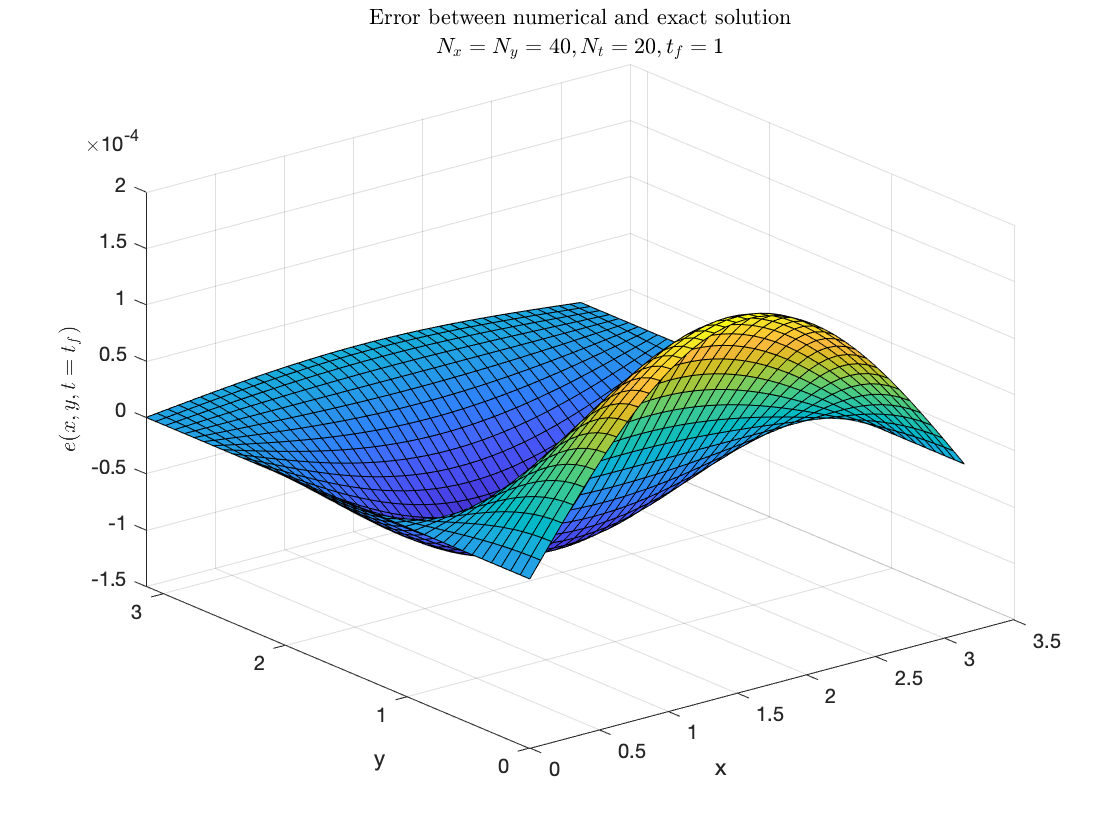
\includegraphics[width=5in]{ADI_ErrPlot.png}
        \caption{Comparison between numerical and exact solution - ADI Scheme}
        \label{fig:ADI_err}
        \end{figure}
        %%
      \item {\color{red}Perform a grid refinement study to verify second-order convergence in both space and time.} \\
      A grid refinement study was performed and the spatial and temporal order of convergence plots are attached in Fig~\ref{fig:ADI_converge}.
      \begin{figure}[htp]
      \centering
      \begin{tabular}{cc}
      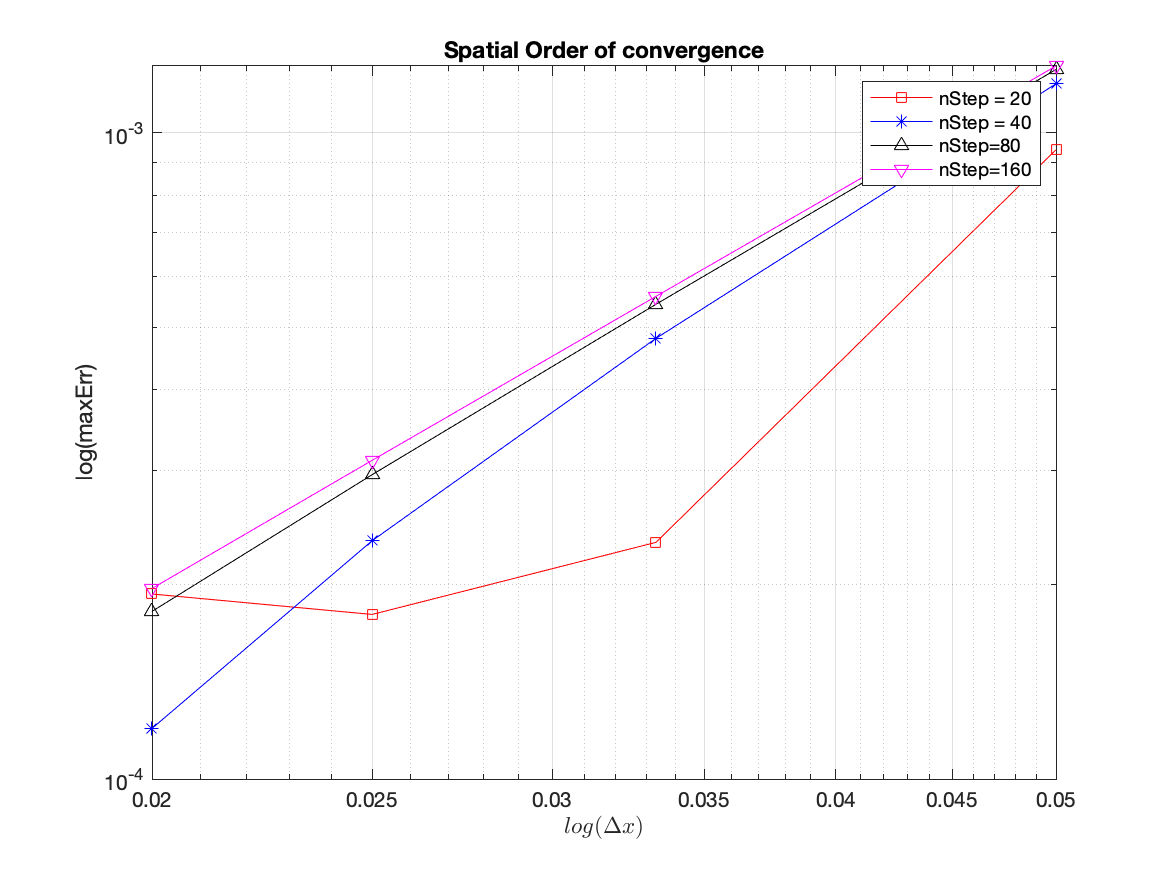
\includegraphics[width=3.3in]{s-ADI_e} & 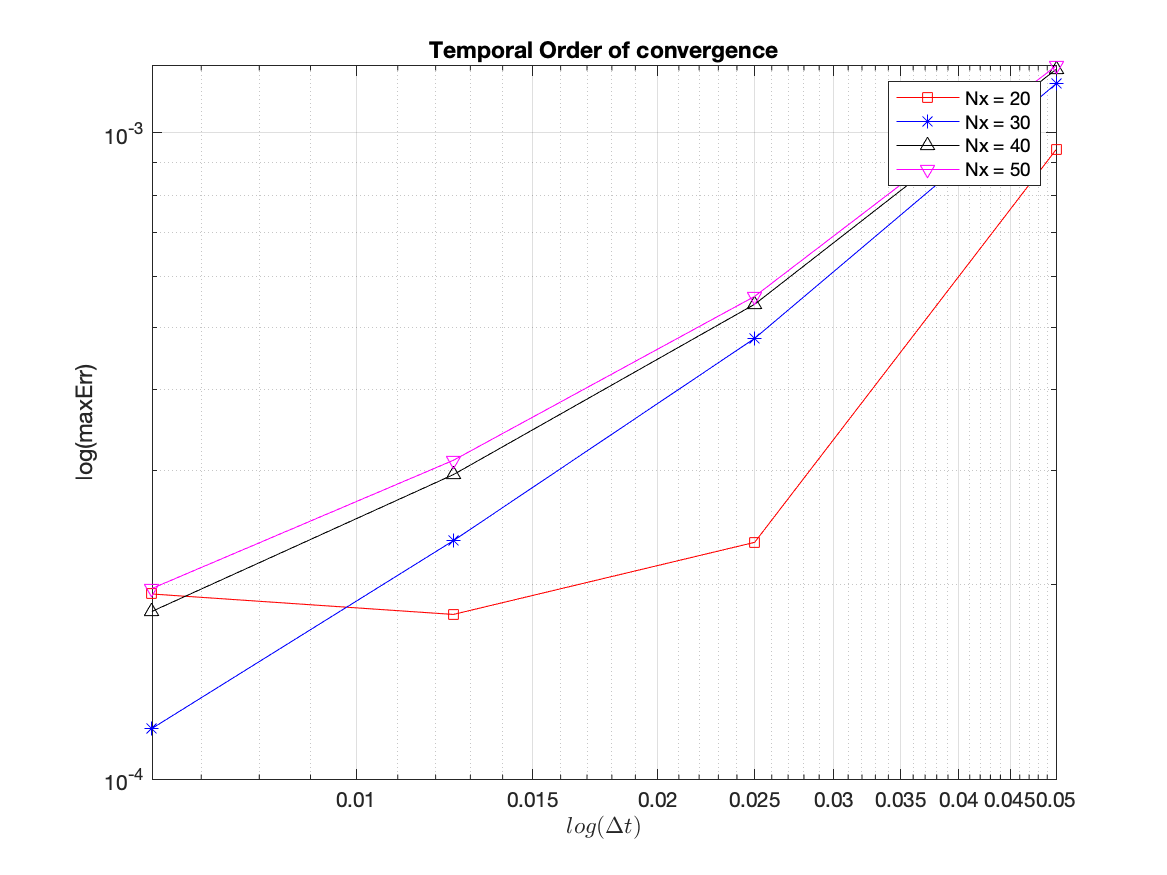
\includegraphics[width=3.3in]{t-ADI_e} \\
      (i) & (ii)
      \end{tabular}
      \caption{Order of Convergence - ADI scheme}
      \label{fig:ADI_converge}
      \end{figure}
      %%
      \item {\color{red}Find a numerical solution using $40$ grid lines in both physical dimensions for the case when }
        \[
          u_0(x,y) = \left\{ 
          \begin{array}{ccc}
            1 & \quad \hbox{ if } & (x-\frac{\pi}{2})^2+(y-\frac{\pi}{2})^2<\frac{1}{2} \\
            0 & \quad \hbox{ else. } &
          \end{array}
          \right.
      \]
      {\color{red}Plot your results at $t=0$, $t=.1$, and $t=.5$}\\
      For this initial function, the results are presented in Fig~\ref{fig:iOpt}
      \begin{figure}
      \centering
      \begin{tabular}{cc}
      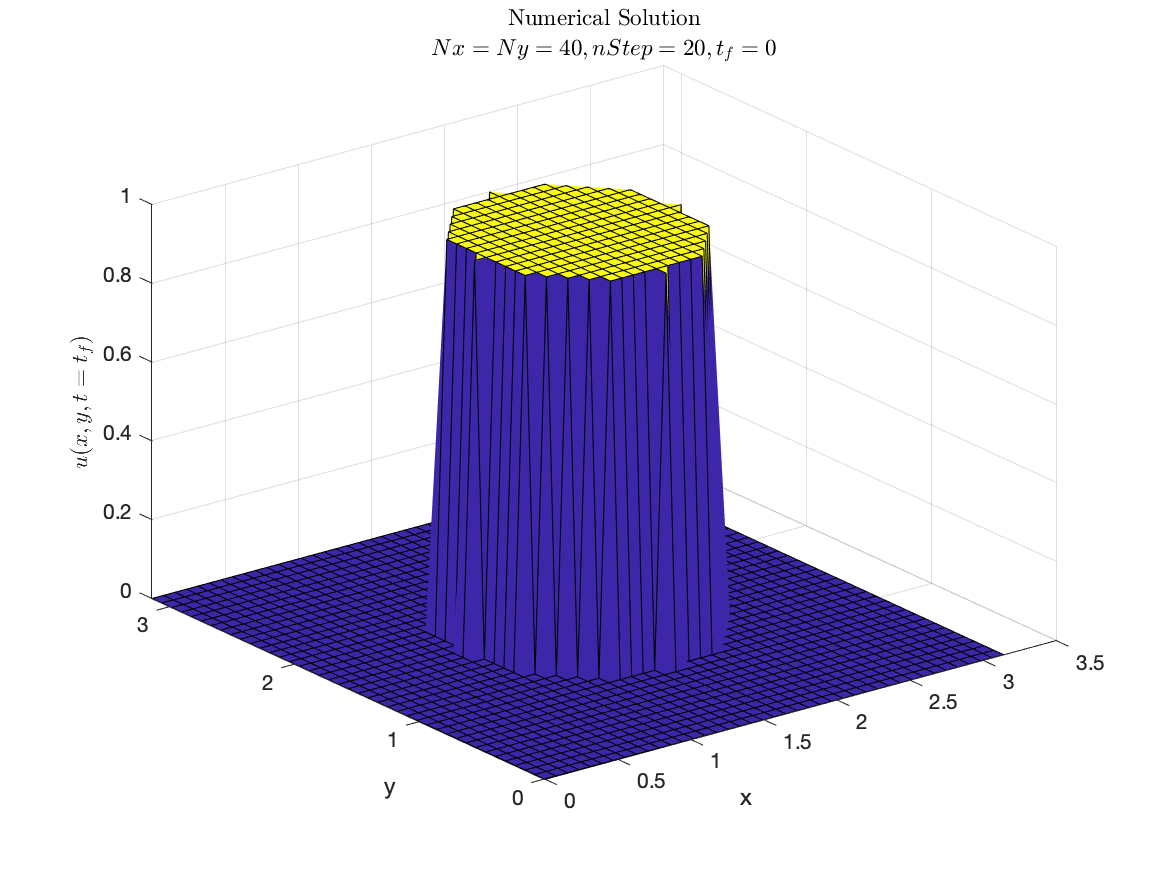
\includegraphics[width=3.5in]{iOpt_1} & 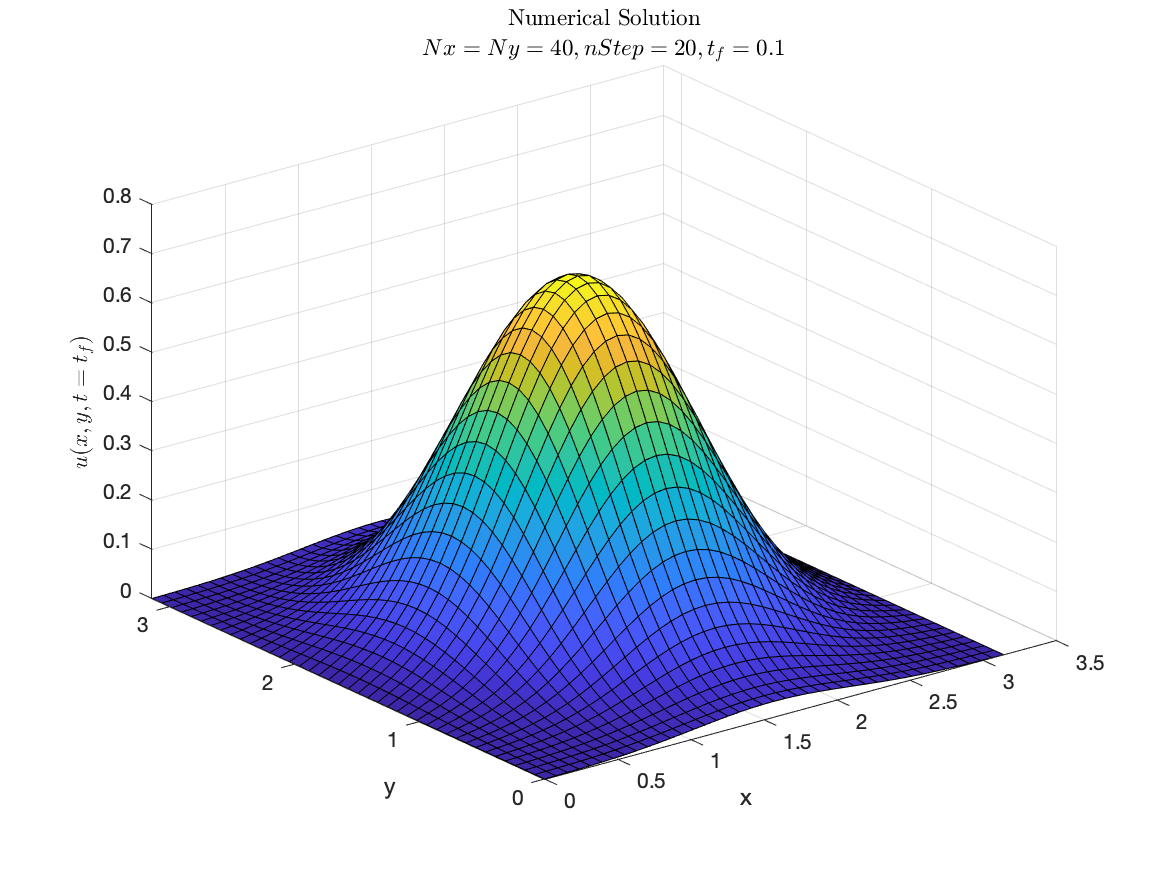
\includegraphics[width=3.5in]{iOpt_2}
      \end{tabular}
      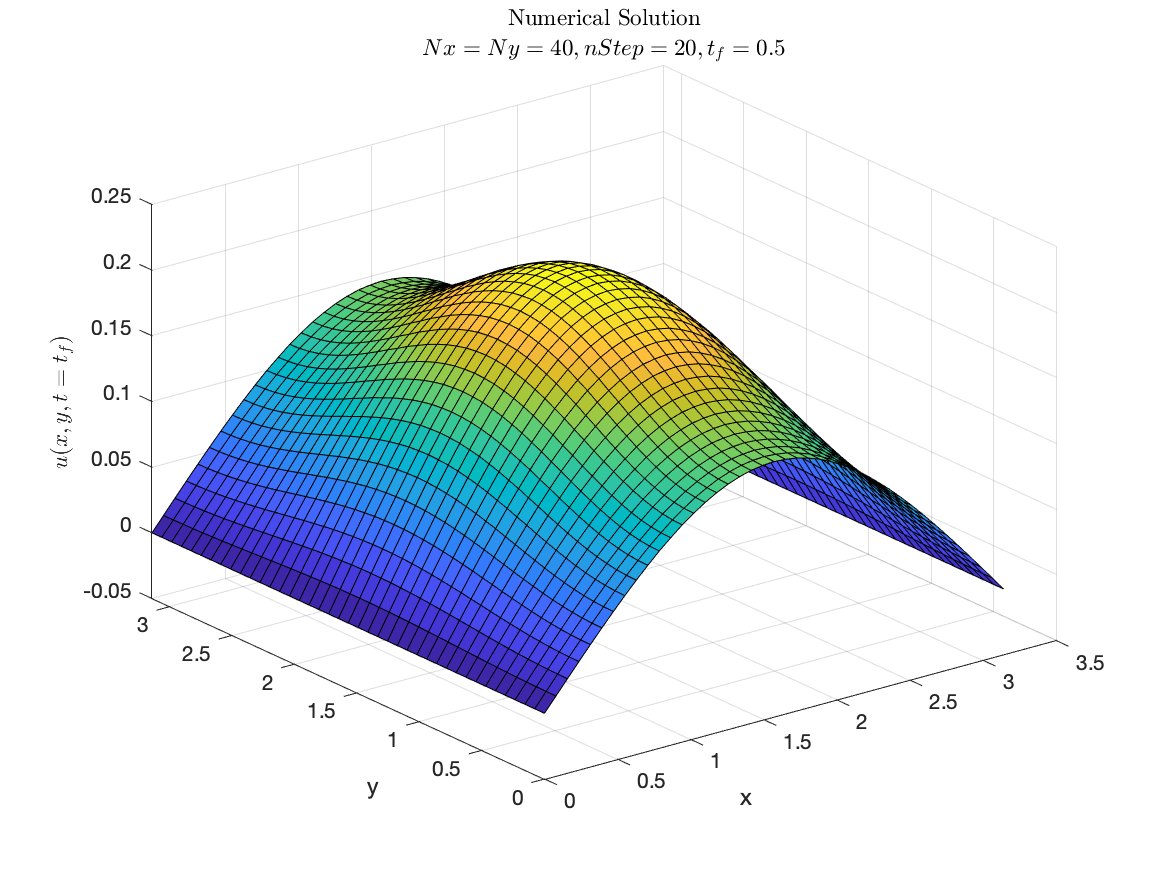
\includegraphics[width=3.5in]{iOpt_3}
      \caption{Numerical Solution at different end times}
      \label{fig:iOpt}
      \end{figure}
    \end{enumerate}
  
\end{enumerate}






\end{document}
